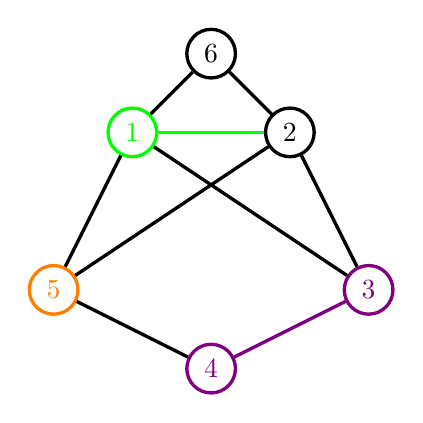
\begin{tikzpicture}
  \node[draw,circle, very thick, color=green] (A) at (1,3) {1};
  \node[draw,circle, very thick] (B) at (3,3) {2};
  \node[draw,circle, very thick, color=violet] (C) at (4,1) {3};
  \node[draw,circle, very thick, color=violet] (D) at (2,0) {4};
  \node[draw,circle, very thick, color=orange] (E) at (0,1) {5};
  \node[draw,circle, very thick] (F) at (2,4) {6};
  \draw[very thick, color=green] (A) -- (B);
  \draw[very thick] (B) -- (C);
  \draw[very thick, color=violet] (C) -- (D);
  \draw[very thick] (D) -- (E);
  \draw[very thick] (A) -- (C);
  \draw[very thick] (B) -- (E);
  \draw[very thick] (A) -- (F);
  \draw[very thick] (B) -- (F);
  \draw[very thick] (A) -- (E);
  
\end{tikzpicture}

